\documentclass[twoside]{book}

% Packages required by doxygen
\usepackage{fixltx2e}
\usepackage{calc}
\usepackage{doxygen}
\usepackage[export]{adjustbox} % also loads graphicx
\usepackage{graphicx}
\usepackage[utf8]{inputenc}
\usepackage{makeidx}
\usepackage{multicol}
\usepackage{multirow}
\PassOptionsToPackage{warn}{textcomp}
\usepackage{textcomp}
\usepackage[nointegrals]{wasysym}
\usepackage[table]{xcolor}

% Font selection
\usepackage[T1]{fontenc}
\usepackage[scaled=.90]{helvet}
\usepackage{courier}
\usepackage{amssymb}
\usepackage{sectsty}
\renewcommand{\familydefault}{\sfdefault}
\allsectionsfont{%
  \fontseries{bc}\selectfont%
  \color{darkgray}%
}
\renewcommand{\DoxyLabelFont}{%
  \fontseries{bc}\selectfont%
  \color{darkgray}%
}
\newcommand{\+}{\discretionary{\mbox{\scriptsize$\hookleftarrow$}}{}{}}

% Page & text layout
\usepackage{geometry}
\geometry{%
  a4paper,%
  top=2.5cm,%
  bottom=2.5cm,%
  left=2.5cm,%
  right=2.5cm%
}
\tolerance=750
\hfuzz=15pt
\hbadness=750
\setlength{\emergencystretch}{15pt}
\setlength{\parindent}{0cm}
\setlength{\parskip}{3ex plus 2ex minus 2ex}
\makeatletter
\renewcommand{\paragraph}{%
  \@startsection{paragraph}{4}{0ex}{-1.0ex}{1.0ex}{%
    \normalfont\normalsize\bfseries\SS@parafont%
  }%
}
\renewcommand{\subparagraph}{%
  \@startsection{subparagraph}{5}{0ex}{-1.0ex}{1.0ex}{%
    \normalfont\normalsize\bfseries\SS@subparafont%
  }%
}
\makeatother

% Headers & footers
\usepackage{fancyhdr}
\pagestyle{fancyplain}
\fancyhead[LE]{\fancyplain{}{\bfseries\thepage}}
\fancyhead[CE]{\fancyplain{}{}}
\fancyhead[RE]{\fancyplain{}{\bfseries\leftmark}}
\fancyhead[LO]{\fancyplain{}{\bfseries\rightmark}}
\fancyhead[CO]{\fancyplain{}{}}
\fancyhead[RO]{\fancyplain{}{\bfseries\thepage}}
\fancyfoot[LE]{\fancyplain{}{}}
\fancyfoot[CE]{\fancyplain{}{}}
\fancyfoot[RE]{\fancyplain{}{\bfseries\scriptsize Generated by Doxygen }}
\fancyfoot[LO]{\fancyplain{}{\bfseries\scriptsize Generated by Doxygen }}
\fancyfoot[CO]{\fancyplain{}{}}
\fancyfoot[RO]{\fancyplain{}{}}
\renewcommand{\footrulewidth}{0.4pt}
\renewcommand{\chaptermark}[1]{%
  \markboth{#1}{}%
}
\renewcommand{\sectionmark}[1]{%
  \markright{\thesection\ #1}%
}

% Indices & bibliography
\usepackage{natbib}
\usepackage[titles]{tocloft}
\setcounter{tocdepth}{3}
\setcounter{secnumdepth}{5}
\makeindex

% Hyperlinks (required, but should be loaded last)
\usepackage{ifpdf}
\ifpdf
  \usepackage[pdftex,pagebackref=true]{hyperref}
\else
  \usepackage[ps2pdf,pagebackref=true]{hyperref}
\fi
\hypersetup{%
  colorlinks=true,%
  linkcolor=blue,%
  citecolor=blue,%
  unicode%
}

% Custom commands
\newcommand{\clearemptydoublepage}{%
  \newpage{\pagestyle{empty}\cleardoublepage}%
}

\usepackage{caption}
\captionsetup{labelsep=space,justification=centering,font={bf},singlelinecheck=off,skip=4pt,position=top}

%===== C O N T E N T S =====

\begin{document}

% Titlepage & ToC
\hypersetup{pageanchor=false,
             bookmarksnumbered=true,
             pdfencoding=unicode
            }
\pagenumbering{alph}
\begin{titlepage}
\vspace*{7cm}
\begin{center}%
{\Large Zip\+Zop }\\
\vspace*{1cm}
{\large Generated by Doxygen 1.8.13}\\
\end{center}
\end{titlepage}
\clearemptydoublepage
\pagenumbering{roman}
\tableofcontents
\clearemptydoublepage
\pagenumbering{arabic}
\hypersetup{pageanchor=true}

%--- Begin generated contents ---
\chapter{Data Structure Index}
\section{Data Structures}
Here are the data structures with brief descriptions\+:\begin{DoxyCompactList}
\item\contentsline{section}{\hyperlink{structclient}{client} \\*Struct representing a connect client in the server }{\pageref{structclient}}{}
\item\contentsline{section}{\hyperlink{structmessage}{message} \\*Struct representing a messege sent by some sender }{\pageref{structmessage}}{}
\item\contentsline{section}{\hyperlink{structsllist}{sllist} \\*A struct representing node in a singly linked list }{\pageref{structsllist}}{}
\end{DoxyCompactList}

\chapter{Data Structure Documentation}
\hypertarget{structclient}{}\section{client Struct Reference}
\label{structclient}\index{client@{client}}


Struct representing a connect client in the server.  


\subsection*{Data Fields}
\begin{DoxyCompactItemize}
\item 
const char $\ast$ \hyperlink{structclient_a99f435ea140a038c3be5e2ab49aa43aa}{name}
\item 
int \hyperlink{structclient_ab7c05dd7a1a5daa5383849d8b3b0ce3f}{sockfd}
\item 
pthread\+\_\+t \hyperlink{structclient_a529fa20e309347262616a00ad0ad3d93}{thread}
\end{DoxyCompactItemize}


\subsection{Detailed Description}
Struct representing a connect client in the server. 

\subsection{Field Documentation}
\mbox{\Hypertarget{structclient_a99f435ea140a038c3be5e2ab49aa43aa}\label{structclient_a99f435ea140a038c3be5e2ab49aa43aa}} 
\index{client@{client}!name@{name}}
\index{name@{name}!client@{client}}
\subsubsection{\texorpdfstring{name}{name}}
{\footnotesize\ttfamily const char$\ast$ client\+::name}

Client name \mbox{\Hypertarget{structclient_ab7c05dd7a1a5daa5383849d8b3b0ce3f}\label{structclient_ab7c05dd7a1a5daa5383849d8b3b0ce3f}} 
\index{client@{client}!sockfd@{sockfd}}
\index{sockfd@{sockfd}!client@{client}}
\subsubsection{\texorpdfstring{sockfd}{sockfd}}
{\footnotesize\ttfamily int client\+::sockfd}

Socket that holds the connection with this client \mbox{\Hypertarget{structclient_a529fa20e309347262616a00ad0ad3d93}\label{structclient_a529fa20e309347262616a00ad0ad3d93}} 
\index{client@{client}!thread@{thread}}
\index{thread@{thread}!client@{client}}
\subsubsection{\texorpdfstring{thread}{thread}}
{\footnotesize\ttfamily pthread\+\_\+t client\+::thread}

The server thread responsible to listen to this client\textquotesingle{}s messages 

The documentation for this struct was generated from the following file\+:\begin{DoxyCompactItemize}
\item 
src/client.\+c\end{DoxyCompactItemize}

\hypertarget{structmessage}{}\section{message Struct Reference}
\label{structmessage}\index{message@{message}}


Struct representing a messege sent by some sender.  


\subsection*{Data Fields}
\begin{DoxyCompactItemize}
\item 
const char $\ast$ \hyperlink{structmessage_ad3b965525fe62cb25162084d97a3f0ff}{content}
\item 
const char $\ast$ \hyperlink{structmessage_a93d4525b657c15744e45ca9504840000}{sender\+\_\+name}
\end{DoxyCompactItemize}


\subsection{Detailed Description}
Struct representing a messege sent by some sender. 

\subsection{Field Documentation}
\mbox{\Hypertarget{structmessage_ad3b965525fe62cb25162084d97a3f0ff}\label{structmessage_ad3b965525fe62cb25162084d97a3f0ff}} 
\index{message@{message}!content@{content}}
\index{content@{content}!message@{message}}
\subsubsection{\texorpdfstring{content}{content}}
{\footnotesize\ttfamily const char$\ast$ message\+::content}

The content of the message \mbox{\Hypertarget{structmessage_a93d4525b657c15744e45ca9504840000}\label{structmessage_a93d4525b657c15744e45ca9504840000}} 
\index{message@{message}!sender\+\_\+name@{sender\+\_\+name}}
\index{sender\+\_\+name@{sender\+\_\+name}!message@{message}}
\subsubsection{\texorpdfstring{sender\+\_\+name}{sender\_name}}
{\footnotesize\ttfamily const char$\ast$ message\+::sender\+\_\+name}

The username of the sender 

The documentation for this struct was generated from the following file\+:\begin{DoxyCompactItemize}
\item 
src/\hyperlink{message_8c}{message.\+c}\end{DoxyCompactItemize}

\hypertarget{structsllist}{}\section{sllist Struct Reference}
\label{structsllist}\index{sllist@{sllist}}


Collaboration diagram for sllist\+:\nopagebreak
\begin{figure}[H]
\begin{center}
\leavevmode
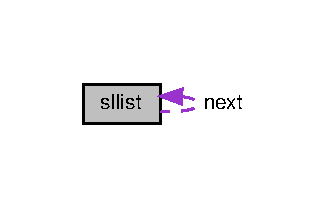
\includegraphics[width=157pt]{structsllist__coll__graph}
\end{center}
\end{figure}
\subsection*{Data Fields}
\begin{DoxyCompactItemize}
\item 
void $\ast$ \hyperlink{structsllist_aba6ff88336afdd0d2a8cb0ce396f79b6}{key}
\item 
struct \hyperlink{structsllist}{sllist} $\ast$ \hyperlink{structsllist_abd84069b1b074a7ac7d94b65672d4fd3}{next}
\end{DoxyCompactItemize}


\subsection{Field Documentation}
\mbox{\Hypertarget{structsllist_aba6ff88336afdd0d2a8cb0ce396f79b6}\label{structsllist_aba6ff88336afdd0d2a8cb0ce396f79b6}} 
\index{sllist@{sllist}!key@{key}}
\index{key@{key}!sllist@{sllist}}
\subsubsection{\texorpdfstring{key}{key}}
{\footnotesize\ttfamily void$\ast$ sllist\+::key}

\mbox{\Hypertarget{structsllist_abd84069b1b074a7ac7d94b65672d4fd3}\label{structsllist_abd84069b1b074a7ac7d94b65672d4fd3}} 
\index{sllist@{sllist}!next@{next}}
\index{next@{next}!sllist@{sllist}}
\subsubsection{\texorpdfstring{next}{next}}
{\footnotesize\ttfamily struct \hyperlink{structsllist}{sllist}$\ast$ sllist\+::next}



The documentation for this struct was generated from the following file\+:\begin{DoxyCompactItemize}
\item 
src/\hyperlink{sllist_8c}{sllist.\+c}\end{DoxyCompactItemize}

%--- End generated contents ---

% Index
\backmatter
\newpage
\phantomsection
\clearemptydoublepage
\addcontentsline{toc}{chapter}{Index}
\printindex

\end{document}
